\documentclass[11pt]{article}
\usepackage[a4paper,margin=2cm]{geometry}
\usepackage{graphicx}
\usepackage{hyperref}
\usepackage{todonotes}
\usepackage{titlesec}
\usepackage{enumitem}
\usepackage{tabularray}
\usepackage{amsmath,amssymb}

\graphicspath{ {./images/} }
\hypersetup{
    colorlinks,
    citecolor=black,
    filecolor=black,
    linkcolor=black,
    urlcolor=black
}
\setlength{\parindent}{0pt}
\titleformat*{\section}{\Large\bf\MakeUppercase}
\titleformat*{\subsection}{\large\bf}


\begin{document}

\begin{titlepage}
    \begin{center}
        \vspace*{1cm}

        \textbf{\LARGE Inteligência Artificial}
        \vspace{0.5cm}

        \Large Resumo
        \vspace{1.5cm}

        \textbf{Rafael Rodrigues}
        \vfill
        LEIC \\
        Instituto Superior Técnico \\
        2022/2023
    \end{center}
\end{titlepage}

\tableofcontents

\newpage
\section{Introduction}

A Inteligência Artificial pode ser vista de 4 perspetivas diferentes, como ilustradas abaixo:

\begin{tabular}[t]{ | l | c | c | }
    \hline
        & Desempenho Humano & Racionalidade \\\hline
    Processos e Raciocínio & Pensar como os humanos & Pensar racionalmente \\\hline
    Comportamento & Atuar como os humanos & Atuar racionalmente \\\hline
\end{tabular}
\vspace{10pt}

A perspetiva seguida na cadeira é a última apresentada, focando-se no estudo de agentes racionais capazes de, tal como o nome sugere, \textbf{atuar racionalmente}.

\subsection{Acting humanly: The Turing Test approach}

Esta abordagem é baseada nos pressupostos do \textbf{Testes de Turing}, o teste é passado se um humano não conseguir distinguir se está a responder a perguntas (ou a interagir) com um humano ou computador.\vspace{10pt}

Um computador, para passar a este teste teria de ter as seguintes capacidades:
\begin{itemize}[topsep=4pt, itemsep=0pt]
    \item \textbf{Capacidade de processar língua natural} - comunicar
    \item \textbf{Representação de conhecimento} - guardar conhecimento
    \item \textbf{Raciocínio automático} - usar o conhecimento para responder
    \item \textbf{Aprendizagem} - adaptar-se
\end{itemize}

\subsection{Thinking Humanly: The Cognitive Modeling Approach}

Para esta abordagem é necessário compreender como é que os humanos pensam e não só o que pensam. Existem 2 formas de fazer isto:
\begin{itemize}[topsep=4pt, itemsep=0pt]
    \item \textbf{Introspeção}
    \item \textbf{Experiências psicológicas}
\end{itemize}
O campo da ciência cognitiva junta os modelos computacionais de IA com as técnicas
experimentais de psicologia para criar teorias precisas e testáveis da mente humana. Quando se tem uma teoria precisa sobre o funcionamento da mente, podemos implementá-la e testar.

\subsection{Thinking Rationally: The “laws of thought” approach}

Esta abordagem é baseada em \textbf{lógica} - que faz uso de regras e notação específicas para traduzir conhecimento.\vspace{10pt}

Existem algumas barreiras a esta abordagem como:
\begin{itemize}[topsep=4pt, itemsep=0pt]
    \item É difícil traduzir conhecimento informal e codificá-lo em lógica.
    \item É fácil esgotar os recursos computacionais se não existir nenhum guia da resolução do problema.
\end{itemize}

\subsection{Acting Rationally: The rational agent approach}

O \textbf{comportamento racional} é traduzido em tomar a decisão correta - definida como aquela que maximiza a expetativa de alcançar um objetivo.

\newpage
\section{Intelligent Agents}

\subsection{Agents and Environments}

Um \textbf{agente} é tudo o que é capaz de captar/perceber o \textbf{ambiente} onde se encontra através de \textbf{sensores} e atuar nesse ambiente através de \textbf{atuadores}. Deve ser \textbf{autónomo}, ou seja, capaz de agir de forma independente de outros agentes e do utilizador.\vspace{10pt}

Uma \textbf{sequência de perceções} é a história completa de tudo o que agente alguma vez percebeu.\vspace{10pt}

Em geral, a escolha de ação de um agente a qualquer instante pode depender de toda a sequência de perceções observada até a data, mas não de algo que ele ainda não percecionou.\vspace{10pt}

Matematicamente, dizemos que o comportamento de um agente é descrito como a \textbf{função agente} que mapeia uma sequência de perceções numa ação. O \textbf{programa agente} é uma implementação concreta executada num sistema físico.

\subsection{Good Behavior: The Concept of Rationality}

Por cada sequência de perceções possível, um \textbf{agente racional} deve selecionar uma ação que é suposto \textbf{maximizar a sua medida de desempenho}, dada a informação disponibilizada pela sequência de perceções e eventualmente pelo conhecimento que o agente possui.\vspace{10pt}

\textbf{Medida de desempenho}: critério objetivo que mede o sucesso do comportamento do agente.\vspace{10pt}

A escolha da ação dependerá do conhecimento adquirido até à data, e não do conhecimento do resultado da ação à priori. Diz-se por isso que um agente deve aprender e ser \textbf{autónomo}.

\subsection{The Nature of Environments}

Os ambientes são os problemas para os quais agentes racionais são a solução.

Um agente pode ser caracterizado pelo acrónimo PEAS:
\begin{itemize}[topsep=4pt, itemsep=0pt]
    \item Performance
    \item Environment
    \item Atuadores
    \item Sensores
\end{itemize}

\subsubsection{Tipos de Ambientes}

\begin{itemize}
    \item \textbf{Observável vs Parcialmente Observável}

    Os sensores do agente dão acesso ao estado completo do ambiente em cada instante de tempo, pelo que não é necessário manter um estado interno sobre o mundo. Quanto mais observável é um ambiente mais fácil a criação de agentes que nele operem.

    \item \textbf{Determinístico vs Estocástico}

    Se o próprio estado do ambiente é completamente determinado pelo estado atual e da ação do agente, então estamos num ambiente determinístico. Num ambiente estocástico há uma probabilidade de incerteza associada. Se um ambiente é sempre determinístico exceto para ações de outros agentes, então o ambiente é \textbf{estratégico}.

    \item \textbf{Episódico vs Sequencial}
    
    A experiência do agente está divida em episódio atómicos. Em cada episódio o agente perceciona e depois executa uma ação. O próximo episódio não depende no anterior. Em ambientes sequenciais, a decisão atual pode afetar as próximas.
    
    \item \textbf{Estático vs Dinâmico}
    
    Um ambiente estático é aquele em que o ambiente não é alterado enquanto o agente decide que a ação vai tomar. Um ambiente semi-dinâmico permanece inalterado com a passagem do tempo mas a qualidade do desempenho do agente é alterada. Um ambiente dinâmico está em constante alteração pelo que as ações dos agentes podem falhar frequentemente.
    
    \item \textbf{Discreto vs Contínuo}

    Num ambiente discreto há um número restrito de estados, ações e perceções enquanto que num agente contínuo o ambiente está em constante mudança.

    \item \textbf{Agente único vs Multi-agente}
    
    Só existe um agente no ambiente.
\end{itemize}

\subsection{The Structure of Agents}

\begin{itemize}
    \item \textbf{Agentes de Reflexos Simples}
    
    Estes agentes atuam com base na sua \textbf{perceção atual}. Não operam bem em ambientes parcialmente observáveis.

    \item \textbf{Agentes de Reflexos baseados em Modelos}
    
    O agente tem um estado interno, que depende do seu histórico de perceções, manter informações do ambiente que não consegue perceber atualmente.

    \item \textbf{Agentes baseados em Objetivos}
    
    O agente atua para atingir o seu objetivo.

    \item \textbf{Agentes baseados em Utilidade}
    
    Os agentes baseados em utilidade têm uma função de utilidade que permite estabelecer preferências entre sequências de estados que permitem atingir os mesmos objetivos. Este agente toma as decisões baseadas na utilidade esperada dos resultados esperados.

    \item \textbf{Agentes com Aprendizagem}
    
    A aprendizagem permite um agente operar num ambiente inicialmente desconhecido e tornar-se mais competente. 

    Um agente com aprendizagem pode ser dividido em 4 componentes conceituais:
    \begin{itemize}[topsep=0pt, itemsep=0pt]
        \item \textbf{Elemento de aprendizagem}: torna o agente mais eficiente.
        \item \textbf{Elemento de desempenho}: seleciona as ações do agente.
        \item \textbf{Elemento de crítica}: dá feedback ao elemento de aprendizagem  e determina se o elemento de performance deve ser modificado no futuro.
        \item \textbf{Elemento de geração de problemas}: sugere ações experimentais que podem trazer informação útil.
    \end{itemize}
\end{itemize}

\newpage
\section{Solving Problems By Searching}

\subsection{Problem-Solving Agents}

Em particular, temos que problem-solving agents devem, ao contrário de outros tipos de agentes mais elementares, poder considerar ações futuras (e as respetivas consequências). Ora, tendo um objetivo estabelecido (objetivo esse gerado a partir do estado final onde queremos chegar, tendo em conta um conjunto de medidas de performance), encontrar a forma ótima de o atingir nem sempre é trivial, acabando frequentemente por requerer \textbf{estratégias de procura} adequadas à situação em que o agente se encontra. De forma sucinta, dizemos que essa "forma ótima de o atingir" corresponde à sequência de ações que o agente terá sucessivamente de tomar por forma a satisfazer o objetivo.

\subsubsection{Well-defined problems and solutions}

Um problema pode ser formalmente definido em 5 componentes:
\begin{itemize}[topsep=4pt,itemsep=0pt]
    \item o \textbf{estado inicial}.
    \item as \textbf{ações que o agente pode tomar}, considerando o seu estado atual.
    \item um \textbf{modelo de transição}, que retorna o estado resultante de executar uma dada ação partindo de um certo estado.
    \item um \textbf{teste objetivo}, um teste simples que nos diz se um dado estado é ou não um estado objetivo. 
    \item um \textbf{custo caminho}, uma função que atribui um custo numérico a cada caminho (consideramos aqui caminho como um todo). Este custo está dependente das medidas de performance pretendidas. Note-se que este ponto se refere ao passado,ou seja, o caminho já percorrido.
\end{itemize}\vspace{4pt}

Uma \textbf{solução} para o problema é uma sequência de estados, do estado inicial ao estado objetivo. A qualidade de uma solução é medida pelo seu custo. A \textbf{solução ótima} é a que tem menor custo.

\setcounter{subsection}{2}
\subsection{Searching For Solutions}

Com o problema formulado, resolvê-lo passa por encontrar a sequência de ações ótima para chegar ao objetivo. Para tal, utilizamos \textbf{algoritmos de procura}, que pesquisam vários ramos da "árvore da sequência de ações", em busca de uma sequência que satisfaça os objetivos dentro das medidas de desempenho pretendidas. Temos, claro, que cada nó da árvore corresponde a um estado (com a raiz sendo o estado inicial), e que os filhos de um nó correspondem aos estados resultantes de tomar uma ação partindo do estado pai.\vspace{4pt}

Chama-se de \textbf{fronteira} de expansão aos nós gerados que ainda não foram expandidos (ou lista de nós abertos).\vspace{4pt}

Os diferentes \textbf{algoritmos de procura} variam apenas na forma como decidem que nó expandir a seguir. A isto chama-se \textbf{estratégia de procura}.\vspace{4pt}

Para evitar os estados repetidos, guardamos o conjunto dos nós já explorados aquando do processamento do algoritmo. Isto significa que todos os nós gerados tem de ser mantidos em memória o que têm uma complexidade espacial exponencial.\vspace{4pt}

\subsubsection{Infrastructure for Search Algorithms}

Para cada nó $n$ de uma árvore, temos a estrutura que contém os seguintes componentes:
\begin{itemize}[topsep=4pt,itemsep=0pt]
    \item $n$.State
    \item $n$.Parent
    \item $n$.Action - ação aplicada ao pai que gerou este nó
    \item $n$.Path-cost - custo $g(n)$ do caminho do estado inicial até este estado
\end{itemize}
To place the visited nodes we typically use queues. These can be FIFO, LIFO (or Stacks) or Priority Queues.

\subsubsection{Measuring problem-solving performance}

As estratégias de procura são avaliadas em 4 aspetos:
\begin{itemize}[topsep=4pt,itemsep=0pt]
    \item \textbf{Completa} - caso encontre sempre uma solução para o problema proposto, caso exista (e caso não exista, diz que não há solução).
    \item \textbf{Complexidade temporal} - número de nós gerados (note-se que não precisam ser expandidos)
    \item \textbf{Complexidade espacial} - número máximo de nós em memória
    \item \textbf{Ótima} - caso encontre a solução ótima (de menor custo).
\end{itemize}\vspace{4pt}

As complexidades são medidas em termos de:
\begin{itemize}[topsep=4pt,itemsep=0pt]
    \item $\boldsymbol{b}$ - máximo factor de ramificação da árvore
    \item $\boldsymbol{d}$ - profundidade da solução de menor custo
    \item $\boldsymbol{m}$ - máxima profundidade do espaço de estados
\end{itemize}

\subsection{Uninformed Search Strategies}

A procura cega (ou não informada), tal como o nome indica, consiste em fazer uma procura sem informação do que vem a seguir - as estratégias sabem apenas o que a definição do problema lhes transmite, sem qualquer tipo de pista ou heurística que permita saber se uma ação é "mais promissora" que outra.

\subsubsection{Breadth-First Search}

Na \textbf{procura em largura primeiro }o nó raiz é expandido, e depois os seus sucessores, e daí em diante. Usa uma fila \textbf{FIFO} para a fronteira, por isso os nós de menor profundidade são sempre os primeiros a serem expandidos.

O teste objetivo é feito quando o nó é gerado e não quando é expandido.

O \textbf{maior problema} da procura em largura primeiro é o \textbf{espaço} por ter um crescimento exponencial. Ainda assim, o tempo é também um grande factor da considerar.

\subsubsection{Uniform-Cost Search}

A \textbf{procura de custo uniforme} expande sempre o nó $n$ da fronteira que tem o menor custo $\boldsymbol{g(n)}$. Assim, a sua fronteira é uma \textbf{fila ordenada pelo custo} do caminho.

Aqui, o teste objetivo tem de ser feito aquando da expansão, não na geração, já que o primeiro nó que passe o teste objetivo pode não ser o nó com menor custo em relação ao caminho total \textbf{aquando da sua geração}.

\subsubsection{Depth-First Search}

A \textbf{procura em profundidade primeiro} expande sempre primeiro o nó com maior profundidade. A fronteira é uma fila \textbf{LIFO}, em que os sucessores são colocados no início.

Procura percorrer um caminho até ao fim, voltando para trás (backtracking) assim que deixa de haver um caminho possível.

\subsubsection{Depth-Limited Search}

A \textbf{procura com profundidade limitada} tenta resolver o problema do espaço de estados infinito da procura em profundidade criando um limite de profundidade que o algoritmo deve calcular. 

Isto introduz no entanto um novo problema: se o nó-objetivo menos profundo estiver para lá do limite por nós imposto, nunca o vamos encontrar. Neste caso o algoritmo retorna "cut-off", assim sabemos que o limite utilizado não corresponde à profundidade máxima da árvore.

\subsubsection{Iterative Deepening Search}

A \textbf{procura de profundidade iterativa} implementa o algoritmo da procura em profundidade limitada recursivamente, incrementando o limite de profundidade.

Na primeira iteração do algoritmo o \textbf{nó raiz não é expandido}.

\subsubsection{Bidirectional Search}

A \textbf{procura bidirecional} consiste na realização de 2 \textbf{procuras em largura} em simultâneo, uma a começar no estado inicial e outra no estado objetivo. A procura termina quando as duas procuras se encontram, ou seja, têm um estado comum.

\subsubsection{Comparing uninformed search strategies}

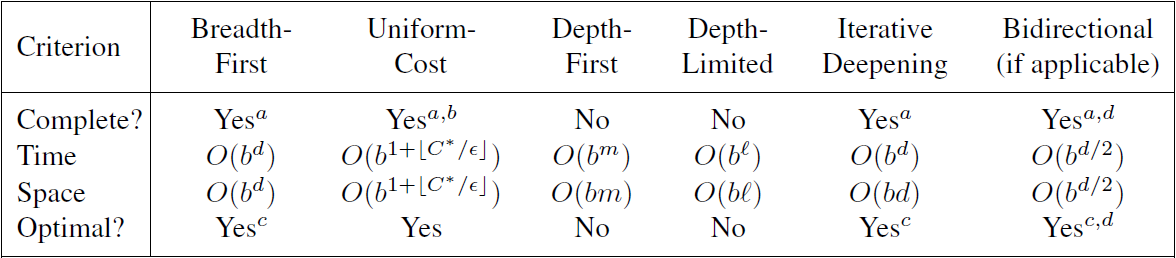
\includegraphics[width=\textwidth]{comparing_uninformed_search_strategies}

$^a$ completa se $b$ é finito \\
$^b$ completa se custo de cada ramo $>$ 0 \\
$^c$ ótima se todos os ramos têm o mesmo custo \\
$^d$ se ambas as direções executam procura em largura primeiro

\subsection{Informed (Heuristic) Search Strategies}

As \textbf{estratégias de procura informadas} são aquelas que usam conhecimento específico do problema para determinar a ordem de expansão dos nós. De um modo geral, estas estratégias baseiam-se na \textbf{procura melhor primeiro}, uma estratégia de procura que recorre a uma \textbf{função de avaliação}, $f(n)$, para escolher a ordem de expansão dos nós.\vspace{4pt}

A função de avaliação é modelada como uma estimativa do custo entre um nó, $n$, e o objetivo. Por norma, poderá ser constituída por algumas componentes principais:
\begin{itemize}[topsep=4pt,itemsep=0pt]
    \item $g(n)$, o custo do caminho percorrido desde o estado inicial até $n$;
    \item $h(n)$, uma \textbf{estimativa} do custo do melhor caminho desde $n$ até ao objetivo;
    \item $h^*(n)$, o \textbf{custo real} do melhor caminho desde $n$ até ao objetivo, isto é, a estimativa exata.
\end{itemize}
Dizemos que $h(n)$ é uma \textbf{função heurística}.

\subsubsection{Greedy Best-First Search}

A \textbf{procura gananciosa} tenta expandir o nó que está \textbf{mais próximo do objetivo}, ou seja, o algoritmo escolhe sempre o nó com a menor função de avaliação.\vspace{10pt}

Função de avaliação: $f(n) = h(n)$

\subsubsection{A* Search}

A \textbf{procura A*} tenta evitar expandir caminhos que já têm um custo muito elevado.\vspace{10pt}

Função de avaliação: $f(n) = g(n) + h(n)$

\subsubsection*{Conditions for optimality: Admissibility and consistency}

Para ser ótima, $h(n)$ tem de ser uma heurística \textbf{admissível}.\\
Uma heurística $h(n)$ é admissível se, para um nó $n$, se verifica que $h(n) \leq h^*(n)$, onde $h^*(n)$ é o custo real do melhor caminho de $n$ até ao objetivo.\\
Isto significa que a heurística \textbf{nunca sobrestima} o custo de atingir o objetivo.\vspace{4pt}

Para além disso a heurística tem também de ser \textbf{consistente}.\\
Dizemos que uma heurística é consistente se, para todo o $n$, para todos os seus sucessores $n'$ gerados por ações $a$, o custo estimado de ir de $n$ ao objetivo for menor ou igual ao custo real de ir de $n$ a $n'$ somado ao custo estimado de ir de $n'$ ao objetivo.
\begin{equation*}
\begin{split}
    f(n') & = g(n) + c(n,a,n') + h(n') \text{ , onde } c(n,a,n') 
                                       \text{ é o custo de } n 
                                       \text{ para } n' \\
          & \geq g(n) + h(n) \\
          & \geq f(n)
\end{split}
\end{equation*}
Podemos, assim, depreender que, numa heurística consistente, $f$ nunca decresce ao longo do caminho.

\subsubsection{Memory-bounded heuristic search}

\subsubsection*{Iterative Deepening A*}

A \textbf{procura iterativa em profundidade de A*}, à semelhança da versão iterativa da DFS tem um limite, neste caso o limite, $l$, baseia-se em $f$ (em vez dos níveis da árvore de procura).\vspace{4pt}

A cada iteração, vamos procurar, usando uma DFS* todos os nós da árvore que possuam $f\leq l$; caso um nó, aquando da sua geração, tenha $f(n)>l$, cortamos-lo da árvore momentaneamente. Levamos a iteração até ao fim, e, quando a acabamos, vamos atualizar o limite para o menor valor de $f$ entre os nós cortados na última iteração. Paramos quando vamos expandir um nó e este passa o teste objetivo.\vspace{10pt}

Função de avaliação: $f(n) = g(n) + h(n)$

\subsubsection*{Recursive Best First Search}

A \textbf{procura melhor primeiro recursiva} procura implementar a procura melhor primeiro em espaço linear (através da recursão). Vamos procurando expandir sempre o nó, dentro dos filhos do nó atual, que tenha menor valor de $f$. Ao mesmo tempo, vamos sempre guardando recursivamente o melhor caminho alternativo ao nó atual - ou seja, o seu irmão ou antepassado com menor valor de $f$. Se nenhum dos seus filhos tiver $f$ menor que esse valor alternativo, passamos então a explorar o nó alternativo guardado (a recursão permite-nos recuperá-lo). A procura termina assim que tentarmos expandir um nó que passa no teste objetivo.\vspace{10pt}

Função de avaliação: $f(n) = g(n) + h(n)$

\subsubsection{Comparing informed search strategies}

\begin{tabular}[t]{ | l | c | c | c | c | }\hline
    Critério & Greedy   & A*          & IDA* & RBFS \\\hline
    Completa & Não      & Sim         &      & Sim, se $b$ finito e custo dos passos $>e$ \\\hline
    Tempo    & $O(b^m)$ & Exponencial &      & Depende da heurística \\\hline
    Espaço   & $O(b^m)$ & Exponencial &      & $O(bd)$ \\\hline
    Ótima    & Não      & Sim         &      & Sim, se $h(n)$ é admissível     \\\hline
\end{tabular}

\subsection{Heuristic Functions}

\todo{Heuristic Functions}

\subsubsection{The effect of heuristic accuracy on performance}

\todo{The effect of heuristic accuracy on performance}

\newpage
\section{Beyond Classical Search}

\subsection{Local Search Algorithms And Optimization Problems}

Quando temos um problema em que o \textbf{caminho} para o objetivo \textbf{não interessa}, podemos usar \textbf{procura local} que mantém um único estado atual, os caminhos não são memorizados.\vspace{4pt}

As \textbf{vantagens da procura local} são:
\begin{itemize}[topsep=2pt,itemsep=0pt]
    \item Usam memória constante
    \item Conseguem encontrar solução em espaços de estados infinitos
    \item Resolvem bem \textbf{problemas de otimização} - encontrar o estado que maximize/minimize uma função de avaliação - e \textbf{problemas de reparação} - estado inicial completo mas não satisfaz as restrições do problema, encontra estado que satisfaça as restrições.
\end{itemize}
\vspace{4pt}

As \textbf{desvantagens} são:
\begin{itemize}[topsep=2pt,itemsep=0pt]
    \item Não podem ser aplicadas quando precisamos de caminho
    \item Não são normalmente completas/ótimas pois ficam presas nos máximos locais
\end{itemize}

\subsubsection{Hill-climbing search}

O \textbf{algoritmo trepar-a-colina} é um algoritmo de procura. É um simples ciclo que se move continuamente na direção de um valor melhor. Termina quando nenhum sucessor têm valores melhores. Não guarda árvore de procura e não olha para além dos vizinhos imediatos.\vspace{4pt}

Este algoritmo tem problemas como:
\begin{itemize}[topsep=2pt,itemsep=0pt]
    \item \textbf{Máximos locais} - pico mais elevado que os seus vizinhos mas mais baixo que o máximo global.
    \item \textbf{Cumes} - sequência de máximos locais.
    \item \textbf{Planaltos} - zona do espaço de estados onde a função de avaliação é plana.
\end{itemize}
\vspace{10pt}

Podemos resolver este problema com variantes do Hill Climbing:
\begin{itemize}[topsep=2pt,itemsep=0pt]
    \item \textbf{Trepar-a-colina estocástico}
    \begin{itemize}[topsep=0pt,itemsep=0pt]
        \item Escolhe aleatoriamente de entre sucessores melhores que estado atual.
        \item Probabilidade de seleção varia em função do valor da melhoria.
    \end{itemize}
    \item \textbf{Trepar-a-colina melhor primeiro}
    \begin{itemize}[topsep=0pt,itemsep=0pt]
        \item Gera os sucessores aleatoriamente até encontrar o primeiro com
        valor melhor que o estado atual (conveniente quando há muitos sucessores).
    \end{itemize} 
    \item \textbf{Trepar-a-colina com começo aleatório}
    \begin{itemize}[topsep=0pt,itemsep=0pt]
        \item Conduz uma séria de procuras a partir de diferentes estados
        iniciais, gerados aleatoriamente. Pára quando encontra o objetivo.
        \item Se $p$ for a probabilidade de sucesso de cada procura o número esperado de tentativas é $1/p$.
        \item Converge rapidamente para uma solução.
        \item É recomendada quando o espaço de estados tem poucos máximos locais e planaltos.
    \end{itemize}
\end{itemize}
\vspace{4pt}

O \textbf{estocástico e melhor primeiro não resolvem} o problema dos máximos locais.

\subsubsection{Simulated annealing}

A procura por \textbf{simulated annealing} baseia-se em tentar fazer com que os estados saiam de máximos ou mínimos locais, "abanando-os". "Abanar" os estados consiste, aqui, em escolher (por vezes) estados com valor objetivo pior do que o que temos atualmente, por forma a procurar sair de máximos/mínimos locais em direção ao global. Esta escolha é feita da seguinte maneira:
\begin{itemize}
    \item Se gerarmos um vizinho com valor objetivo maior que o que temos atualmente, escolhemo-lo.
    \item Caso geremos um vizinho com valor objetivo menor que o que temos atualmente, existe a \textbf{possibilidade} de o escolhermos na mesma: temos, contudo, de ter cuidado para não nos afastarmos demasiado dos extremos locais que já encontrámos, ficando ainda mais longe de encontrar extremos globais, pelo que a probabilidade (sempre menor que 1) de escolher estes vizinhos diminui à medida que o movimento se aproxima cada vez mais dos extremos globais - isto é, se nos estivermos a aproximar "do que queremos", não faz tanto sentido ir noutra direção como fazia inicialmente, quando estávamos longe e qualquer abanão podia surtir efeitos positivos.
\end{itemize}

\subsubsection{Local beam search}

Na \textbf{procura local em banda} optamos por gerar $k$ estados iniciais, todos eles aleatórios. Se algum deles for estado-objetivo, paramos. Caso contrário, vamos ver todos os vizinhos dos $k$ estados, e escolhemos os $k^*$ melhores estados, entre todos os vizinhos que gerámos. Este processo é realizado iterativamente até que encontremos um estado-objetivo.\vspace{10pt}

Podemos, eventualmente, chegar a situações em que os $k$ estados que temos em mãos são pouco diversos. Para nos ajudar a combater este problema, existe a variante \textbf{estocástica} da procura local em banda, onde em vez de escolhermos sempre os kk melhores vizinhos dos estados atuais, escolhemos $k$ vizinhos de forma aleatória. Esta abordagem permite uma maior diversidade no conjunto de estados que vamos explorando.

$^*$Note-se que caso um dos estados, seja ele $K$, gere $\frac{K}{2}$ vizinhos fantásticos e todos os outros, para todos os outros estados, sejam medíocres, não vamos apenas escolher 1 vizinho por estado: vamos escolher os $\frac{K}{2}$ vizinhos de $K$, e depois outros $\frac{K}{2}$ vizinhos entre o resto dos medíocres.

\subsubsection{Genetic algorithms}

Correspondem a algoritmos baseados na procura em banda estocástica, referida acima, e na ideia da "seleção natural" associada à genética. Começamos com uma população inicial, com $k$ estados (ou indivíduos). Estes indivíduos vão eventualmente reproduzir-se, por forma a dar continuidade à espécie (leia-se, vamos gerar os estados vizinhos), e eventualmente vamos gerando indivíduos "melhores", tal como dita a teoria da evolução - as mutações positivas mantêm-se, da mesma maneira que vamos sempre procurar estados que estejam a "ir na direção certa". Esta noção de estados melhores e piores pode ser quantificada segundo uma função, a \textit{fitness function}, onde os melhores estados recebem os valores mais altos. Vamos cruzando estados pais, mantendo propriedades iguais entre os mesmos, procurando ainda verificar se certas alterações levam ou não a resultados melhores, em busca do estado que corresponde a uma solução.\vspace{10pt}

Este tipo de algoritmos pode, ainda, variar considerando várias componentes:

\begin{itemize}[topsep=2pt,itemsep=0pt]
    \item O tamanho da população pode, claro, ser infinitamente variável;
    \item A representação de um estado é também arbitrária: tanto podemos ter strings sobre alfabetos $\{0,1\}$, como qualquer alfabeto numérico, entre outros;
    \item A quantidade de "pais" - acima foram referidos dois pais, mas podemos ter um (sendo essa abordagem a procura em banda estocástica clássica) ou mesmo mais que dois pais;
    \item O próprio processo de seleção, que não tem necessariamente de ter uma relação direta com a fitness function (podendo ser mais aleatório), entre outras.
\end{itemize}

\subsection{Local Search in Continuous Spaces}

\subsection{Searching with Nondeterministic Actions}

Em cenários reais, as nossas ações podem ter mais do que um resultado possível. Vamos, portanto, ter de adaptar a nossa noção de modelo de transição, passando esta a retornar um \textbf{conjunto de estados} que podem resultar de aplicar uma ação $a$ a um estado $s$.

\subsubsection{AND-OR search trees}

São árvores com dois tipos de nós, onde:
\begin{itemize}[topsep=2pt,itemsep=0pt]
    \item os nós OR correspondem a ações.
    \item os nós AND correspondem a estados.
\end{itemize}\vspace{4pt}

A lógica por detrás destas árvores é, então, simples de entender: partindo de nós AND, vemos que ações podemos executar a partir deles, e geramos os nós correspondentes (que vão ser seus filhos) - os nós OR. Posteriormente, verificamos os estados resultantes de aplicar a ação em OR ao pai AND, e daí resultam os filhos de OR: os tais estados resultantes, um conjunto de nós AND.\vspace{10pt}

Neste tipo de árvores, \textbf{todas as folhas são objetivos}. Mais ainda, caso encontremos um estado repetido seguindo um dado caminho, podemos dizer que \textbf{entrámos em ciclo}, retornando \textit{failure}.

\subsubsection{Try, try again}

Existem cenários onde temos de utilizar ciclos para atingir a solução pretendida. Depreende-se, então, que ciclos causados "aleatoriamente" são aceitáveis, e que qualquer outro tipo deve ser rejeitado. 

\subsection{Searching with Partial Observations}

Em ambientes parcialmente observáveis a procura vai tratar, em vez de um conjunto de estados palpáveis/completamente observáveis, de um \textbf{conjunto de crenças} do agente. Tem um conjunto de componentes diferente do que foi visto até agora:
\begin{itemize}
    \item Um conjunto de estados, o \textbf{espaço de crenças}: contém todos os subconjuntos de estados físicos do problema original;
    \item Um \textbf{estado inicial} - por norma, encontra-se inicialmente \textbf{cheio}, já que, na pior das hipóteses, não temos qualquer informação sobre o que nos rodeia (tendo, portanto, de considerar qualquer cenário como possível). Na prática, costumamos ter algumas pistas quanto ao estado inicial;
    \item Um \textbf{conjunto de ações}, que corresponde ao conjunto de todas as ações que podemos fazer partindo de qualquer um dos estados do espaço de crenças;
    \item Um \textbf{modelo de transição}, que difere entre as versões determinista e não-determinista. Num problema $P$, para uma dada crença $b$, a versão determinista dita que a crença $b'$, resultante de aplicar uma qualquer ação $a$ será dada por:
    \begin{equation*}
        b'=result(b,a)=\{s':s'=s\in b\cap s'\in result_p(s,a)\}
    \end{equation*}
    Por outro lado, a versão não-determinista dita que:
    \begin{equation*}
    \begin{split}
        b' = result(b,a) & = \{s':s'=s\in b\cap s'\in result_p(s,a)\cup b\} \\
                         & = \bigcup_{s\in b} result_p(s,a)
    \end{split}
    \end{equation*}
    O modelo de transição tem três etapas: inicialmente, a fase da \textbf{previsão}, onde vai calcular as crenças resultantes da ação que vai tomar. De seguida, caso esteja num ambiente parcialmente observável, utiliza os seus sensores e a informação obtida para atualizar o seu espaço de crenças.
    \item O \textbf{teste objetivo}, que aqui tem um senão: só é garantido que estamos no objetivo se todo o nosso espaço de crenças assim o afirmar - isto é, se todos os estados do nosso espaço de crenças satisfizerem o objetivo; caso contrário, \textbf{possivelmente} alcançámos o objetivo, sem qualquer garantia.
\end{itemize}

\subsection{Online Search Agents and Unknown Environments}

Quando não conhecemos o ambiente que nos envolve, e existem penalizações (sejam elas artificiais ou naturais) por tempos de computação demasiado longos, pode fazer sentido intervalar a procura com ações, em vez de seguir sempre a mesma linha de procura até agora abordada: observamos o ambiente atual e o que sabemos sobre ele, calculamos a próxima ação a tomar por forma a atingir mais rapidamente o objetivo, e executamos essa mesma ação. Esta navegação consegue assemelhar-se, de vez em quando, a uma procura às cegas.\vspace{4pt}

Note-se que esta abordagem tem particular utilidade no âmbito da exploração - é bastante provável que um agente, procurando às cegas, chegue ao fim tendo procurado a vasta maioria do ambiente que o envolve. Quanto à velocidade a que chega ao objetivo, contudo, é obviamente pior: uma procura pensada, em que conhecemos o ambiente e podemos prever o resultado das nossas ações tem todo um outro nível de "curadoria" que nos permite chegar mais eficientemente ao objetivo.\vspace{4pt}

Abordámos, sem saber, um tipo de procura (local) cega mais acima: \textbf{hill climbing}, se pensarmos bem, mantém apenas informação sobre os seus vizinhos diretos, e não tem noção do meio que o envolve sem ser o que imediatamente o rodeia. Podemos, contudo, \textbf{adicionar memória} a hill climbing, por forma a tornar esta procura mais inteligente: guardamos uma estimativa de quanto custa chegar ao objetivo, partindo de cada estado que já foi visitado.\vspace{4pt}

O agente, aqui, utiliza o que sabe sobre a sua envolvência e, enquanto explora, vai guardando a nova informação sobre o ambiente que o rodeia. Assim que se apercebe que pode seguir um caminho melhor que o anterior, escolhe-o. A esta procura, hill climbing com memória, dá-se também o nome de \textbf{\textit{Learning Real-Time A*}}, $LRTA^*$. Dizemos que $LRTA^*$ opera segundo o princípio de \textbf{otimismo sob incerteza}: ao contrário da versão clássica de hill climbing, aqui o agente é encorajado a explorar o ambiente que o rodeia.


\newpage
\section{Adversarial Search}

\subsection{Games}

Na teoria de jogos, um ambiente multi-agente é um jogo sendo os agentes competitivos ou cooperativos. Em IA, os jogos mais comuns são especializados - determinísticos, em turnos, 2 jogadores, jogos de soma 0 (valores da utilidade são sempre iguais e opostos).\vspace{4pt}

Vamos considerar que existem 2 jogadores, um MAX e outro MIN. O MAX joga primeiro. No final do jogo, o vencedor ganha pontos e o adversário é penalizado (ou empate).\vspace{4pt}

O jogo em si tem várias componentes-base:
\begin{itemize}[topsep=4pt, itemsep=0pt]
    \item Um estado inicial, $S_0$, que corresponde à configuração inicial do mesmo.
    \item Uma função, $player(s:state)$, que especifica o jogador que vai jogar no estado em questão.
    \item Uma função, $action(s:state)$, que retorna todas as jogadas possíveis para o estado em questão.
    \item Uma função, $result(s:state,\ a:action)$, que, tal como abordado em secções anteriores, corresponde ao modelo de transição do jogo, que define o estado resultante de realizar uma jogada $a$ sob um estado $s$.
    \item No lugar do $goal\_test$, abordado anteriormente, vamos ter uma função $terminal\_test$ (que funciona de forma praticamente igual): retorna true caso o jogo esteja num estado terminal, e false caso contrário.
    \item Por fim, uma função $utility(s:state,\ p:player)$, que especifica a pontuação atribuída a um jogador $p$ caso o jogo termine num estado terminal $s$.
\end{itemize}

O estado inicial e as funções ações e resultado definem a árvore do jogo. Os nós são estados e os ramos são jogadas.

\subsection{Optimal Decisions in Games}

Um dos algoritmos clássicos de procura em jogos é o Minimax.\vspace{4pt}

\subsubsection{The minimax algorithm}

O funcionamento do algoritmo Minimax é relativamente simples: cada agente vai sempre escolher a jogada que maximiza o valor minimax, que corresponde ao melhor valor para a função de utilidade contra as melhores jogadas do adversário: assumimos, portanto, que o adversário escolhe sempre a melhor jogada possível. \vspace{4pt}

Colocando por palavras, temos que MIN vai sempre tentar escolher a jogada que minimiza as hipóteses de MAX ganhar. Assim sendo, de entre todas as jogadas que MIN idealmente fará, MAX vai tentar maximizar as suas próprias hipóteses de ganhar, escolhendo a jogada com maior valor minimax.

\subsubsection{Optimal decisions in multiplayer games}

Podemos generalizar o funcionamento do algoritmo para $n$ agentes. Para tal, vamos guardar um \textbf{vetor de valores Minimax}, em vez de um valor só, e cada jogador vai, idealmente, escolher a jogada que mais o beneficia de entre todas as possíveis, mantendo, claro, guardados também os valores que cada jogada terá para os outros agentes: havendo uma quantidade arbitrária de jogadores, cada um deles acaba por não se preocupar tanto com "estragar o jogo ao outro" como com "fazer o melhor possível com o próprio jogo". As estratégias ótimas podem, naturalmente, traduzir-se em alianças informais entre vários jogadores.

\subsection{Alpha-Beta Pruning}

Uma forma de otimizar o algoritmo Minimax é cortando ramos da árvore, utilizando uma técnica chamada \textbf{Alpha-Beta Pruning}. Esta técnica remove ramos irrelevantes à decisão final.

Temos que o $\alpha$ de um nó $n$ é o valor da melhor escolha para o jogador MAX encontrada em qualquer ponto da decisão ao longo do caminho para $n$. Temos que $\beta$ é o valor da melhor escolha para o jogador MIN encontrada em qualquer ponto de decisão ao longo do caminho para $n$.

\subsubsection{Move ordering}

Os cortes dependem dos valores de alfa e beta. Portanto vamos escolher primeiro os
sucessos que atualizem alfa e beta da melhor maneira possível. O que significa no nó MAX visitar primeiro o sucessor com maior valor e nó MIN visitar primeiro o sucessor com menor valor.
Infelizmente, não sabemos o valor minimax de um nó antes de o visitar. Como é que podemos escolher qual o melhor a visitar primeiro sem o visitar? Estimar com uma \textbf{heurística}.

\subsection{Imperfect Real-Time Decisions}

Mesmo com os cortes, a procura alfa-beta ainda \textbf{tem de percorrer até à profundidade máxima} pelo menos uma parte da árvore de jogo, o que não é eficiente. Foi proposto que os programas devam cortar a árvore e acabar a procura mais cedo,utilizando uma \textbf{função de avaliação heurística} que torna nós não-terminais em folhas terminais. Por outras palavras substitui-se a função $utility$ por uma avaliação heurística, \textbf{eval}.

\subsubsection{Evaluation functions}

A função de avaliação $eval$ devolve uma estimativa da utilidade do estado.
\begin{enumerate}[topsep=4pt, itemsep=0pt]
    \item A função de avaliação deve ordenar os estados terminais da mesma forma que a função de utilidade verdadeira.
    \item A computação têm de ser rápida.
    \item Para estados não terminais, a função de avaliação deve estar fortemente correlacionada com as chances de ganhar.
\end{enumerate}
\vspace{4pt}

Tipicamente, as funções de avaliação são uma soma linear de características do jogo , $f$, associadas a diferentes pesos, $w$.
\begin{equation*}
    eval(s) = w_1f_1(s)+w_2f_2(s)+\ldots+w_nf_n(s)
\end{equation*}
A soma dos valores de diferentes características é razoável embora seja uma assunção demasiado forte pois \textbf{assume que as características são independentes} umas das outras. Atualmente maior parte dos programas usam combinações não-lineares.

\subsubsection{Cutting off search}

De modo a que a heurística $eval$ funcione apenas quando é apropriado cortar a procura, substitui-se a função \textit{terminal\_test} pela função \textit{cutoff\_test} que recebe um estado e a profundidade desse estado e decide se o estado é considerado final (mesmo não o sendo).\vspace{4pt}

Temos ainda o problema da \textbf{aquiescência} (estados inativos, parados, ..). Os estados \textbf{não aquiescentes} no limite devem ser expandidos até que sejam gerados \textbf{estados aquiescentes}. A esta procura adicional chama-se \textbf{procura aquiescente}.\vspace{4pt}

O \textbf{efeito horizonte} é mais difícil de eliminar. Este surge quando o programa está a lidar com um movimento do oponente que causou danos e que não pode evitar sem ser atrasando certas estratégias. Uma estratégia para resolver isto é a \textbf{extensão singular} - quando é encontrada uma jogada considerada claramente melhor que as jogadas restantes para a mesma posição essa jogada é registada como singular e aumenta-se o limite de procura para os sucessores da jogada singular. Assim, a profundidade da árvore aumenta.

\subsubsection{Forward prunning}

Ao contrário dos cortes $\alpha$-$\beta$, onde temos a garantia de que o que estamos a cortar é irrelevante para o valor da função de avaliação de um nó, aqui vamos procurar "prever" que assim é, sem qualquer garantia de tal ser o caso. Temos duas maneiras principais de os fazer:
\begin{itemize}
    \item \textbf{Procura em Banda/Beam Search} - consideramos, para cada nível, as $n$ melhores jogadas (segundo a função de avaliação associada). Não há garantias de que não estamos a cortar ramos que nos levariam à jogada ótima.
    \item \textbf{Corte Probabilístico/ProbCut} - cortamos não só os ramos que estão garantidamente fora da "janela $(\alpha,\beta)$", como também os que provavelmente estão: usamos a "experiência de procuras anteriores" para determinar a probabilidade de um dado valor a uma dada profundidade estar ou não fora da janela $(\alpha,\beta)$.
\end{itemize}

\subsection{Stochastic Games}

Os jogos estocásticos são os que introduzem o elemento \textbf{sorte}: para além de haver a imprevisibilidade dos movimentos do adversário, existe também a possibilidade da ação que queremos fazer não corresponder à que de facto acontece. É como se no xadrez, para além de termos a dificuldade de fazer a jogada que nos aproxime mais da vitória, ainda tenhamos que lançar um dado para ver que conjunto de jogadas é que podemos fazer em cada ronda. Cada nó vai ter, assim, de estar associado a uma probabilidade, para além da própria "qualidade da jogada": vamos querer combinações que incluam jogadas prováveis e jogadas boas, por forma a tentar ter as melhores previsões possíveis (que nos levem a boas jogadas). A complexidade temporal destes problemas é $O(b^dn^d)$, onde nn corresponde ao número de lançamentos distintos de dados que realizamos. Conseguimos, portanto, atingir profundidades muito menores no mesmo intervalo de tempo.

\newpage
\section{Constraint Satisfaction Problems}

Nesta secção, vamos aprofundar a ideia de estados não atómicos, com conteúdo no seu interior, um \textbf{conjunto de variáveis}: dizemos que chegámos a uma solução para o problema proposto quando todas as variáveis estiverem associadas a valores que satisfaçam as restrições impostas pelo mesmo. Dizemos que os problemas resolvidos desta forma são Problemas de Satisfação de Restrições (do inglês Constraint Satisfaction Problems, \textbf{CSP}). Idealmente, algoritmos de procura que assentem nesta ideia irão progressivamente eliminando ramos da nossa árvore de procura, tornando-a assim mais eficiente.

\subsection{Defining Constraint Satisfaction Problems}

Podemos definir um CSP como um conjunto de três componentes:
\begin{itemize}[itemsep=0pt]
    \item um \textbf{conjunto de variáveis}: seja ele $X=\{X_1,X_2,\cdots,X_n\}$;
    \item um \textbf{conjunto de domínios}, onde um domínio corresponde ao conjunto de valores que podem ser associados a uma variável: seja ele $D=\{D_{x_1},D_{x_2},\cdots,D_{x_n}\}$;
    \item um \textbf{conjunto de restrições}, que especifica todas as combinações possíveis de valores que podemos ser associados às variáveis ao mesmo tempo numa solução correta: seja ele $C$.
\end{itemize}

Temos ainda que as restrições podem ser \textbf{explícitas}, quando especificam diretamente todas as combinações possíveis de valores que podem ser associados às variáveis, ou \textbf{implícitas}, quando o fazem através de expressões matemáticas ou equivalente.\vspace{10pt}

Um estado será, portanto, definido como um conjunto de correspondências entre variáveis e valores, correspondências essas que não deverão violar qualquer das restrições impostas pelo problema. Estas correspondências, ou \textbf{atribuições, podem ser parciais ou completas}.\vspace{4pt}

Uma atribuição diz-se:
\begin{itemize}[topsep=4pt,itemsep=0pt]
    \item \textbf{Completa} - caso todas as variáveis em $X$ tenham um valor associado.
    \item \textbf{Consistente} - caso todas as atribuições respeitem o conjunto $C$.
\end{itemize}\vspace{10pt}

Dizemos que temos em mãos uma \textbf{solução} para o CSP quando temos uma atribuição \textbf{completa e consistente}: não existem variáveis sem atribuições, estando todas elas atribuídas de acordo com o que o problema nos impõe.

\subsubsection{Variations on the CSP formalism}

Os tipos mais simples de CSP envolvem variáveis que tem domínios \textbf{discretos e finitos}. Um domínio \textbf{discreto pode também ser infinito}, como por exemplo um conjunto de inteiros ou strings, neste caso usamos uma \textbf{linguagem de restrições}.\vspace{10pt}

Tipos de restrições:
\begin{itemize}
    \item \textbf{Restrições unárias} - restringem o valor de uma variável.
    \item \textbf{Restrições binárias} - relacionam um par de variáveis.
    \item \textbf{Restrições de ordem superior} - envolvem 3 ou mais variáveis.
    \item \textbf{Restrições globais} - envolvem um número arbitrário de variáveis (por exemplo todas).
    \item \textbf{Restrições de preferência} - ajudam a modelar o problema em volta de um conjunto de coisas que gostávamos que acontecessem (e damos um peso a cada uma, conforme sejamos mais ou menos firmes quanto a que tal aconteça ou não). Todas essas preferências poderão ser introduzidas num conjunto à parte, o \textbf{conjunto de restrições de preferências do problema}, onde cada uma destas preferências seria devidamente pesada e resolvida como um \textbf{problema de otimização de restrições.}
\end{itemize}

\subsection{Constraint Propagation: Inference in CSPs}

Os algoritmos abordados para as procuras cega e informada limitavam-se a andar pela árvore de procura, à procura da "melhor solução" possível para o problema em mãos. No caso de algoritmos baseados em CSPs, para além de podermos fazer uma procura clássica, temos ainda a noção de restrições; mais importante ainda, temos a noção de \textbf{propagação de restrições}, uma forma de fazer inferência quanto a uma dada situação, atualizando progressivamente os caminhos que podemos tomar. As restrições podem ser-nos úteis logo no pré-processamento inicial do problema, podendo, inclusive, fazer com que não tenha de haver procura: num Sudoku fácil, por exemplo, existe sempre um movimento "obrigatório" (leia-se "aquele número tem de estar ali") à medida que vamos avançando no jogo, pelo que o pré-processamento leva a uma propagação sucessiva de restrições que levam a uma solução direta, sem recorrer a procura/tentativas sem garantias.\vspace{4pt}

A propagação tem por objetivo, assim, utilizar as restrições a seu favor por forma a \textbf{reduzir o tamanho dos domínios das variáveis} (idealmente a 1, nunca a 0), garantindo, assim, que "aquela variável tem de estar associada àquele valor para uma solução consistente". Vai, aqui, voltar a ser relevante aquela visualização do problema como um grafo mencionada mais acima.

\subsubsection{Node consistency}

Dizemos que uma variável é \textbf{nó-consistente} caso todos os valores no seu domínio satisfaçam as suas restrições unárias. Adicionalmente, dizemos que um \textbf{grafo} é nó-consistente caso todas as suas variáveis também o sejam.

\subsubsection{Arc consistency}

Dizemos que uma variável é \textbf{arco-consistente} caso todos os valores no seu domínio satisfaçam as suas restrições binárias. Temos que um \textbf{grafo} é arco-consistente caso qualquer variável seja arco-consistente com todas as outras variáveis.\vspace{10pt}

O algoritmo mais conhecido para tratar a consistência de arcos é o AC-3. O seu funcionamento é relativamente simples: mantemos um set de arcos (que inicialmente tem todos os arcos do CSP), e vamos aleatoriamente removendo um arco do set (seja o arco $(X,Y)$); fazemos com que $X$ seja consistente em arco com $Y$, e daí vamos ter três cenários possíveis:
\begin{itemize}
    \item Caso $D_X$ não tenha sido alterado, $X$ já era consistente em arco com $Y$, pelo que o arco é só removido e não acontece nada;
    \item Caso $D_X$ \textbf{tenha visto o seu tamanho reduzido} (com $\left\lvert D_X\right\rvert\neq 0$), adicionamos todos os outros arcos $(X,X_j)$ de volta ao set - temos restrições adicionais, pelo que podemos agora encontrar outras maneiras de reduzir o tamanho do domínio de $X$;
    \item Caso $D_X$ tenha visto o seu domínio reduzido ao \textbf{conjunto vazio}, podemos afirmar que não existe solução consistente para o problema, pelo que o algoritmo retorna \textit{failure}.
\end{itemize}
O algoritmo termina quando verifica que o domínio de uma das variáveis passa a ser o conjunto vazio, retornando failure, ou quando o set de arcos fica vazio, retornando true.

\subsubsection{Path consistency}

A consistência de caminhos permite analisar trios de variáveis em vez de pares.\vspace{4pt}

Um conjunto de 2 variáveis $\{X_i, X_j\}$ é consistente em caminho para uma 3ª variável Xm sse para cada atribuição ${X_i = a, X_j = b}$ consistente com as restrições ${X_i, X_j}$ então têm que existir uma atribuição para $X_m$ que satisfaça as restrições de ${X_i, X_m}$ e ${X_m, X_j}$.

\subsubsection{K-consistency}

Um CSP é $k$-consistente se, para qualquer conjunto de $k-1$ variáveis e para qualquer atribuição consistente para essas variáveis, existir uma atribuição consistente para a variável $k$.\\
Um CSP diz-se \textbf{fortemente k-consistente} se é $k$-consistente, e $(k-1)$-consistente, $\ldots$, $1$-consistente.

\subsubsection{Global constraints}

Restrições globais ocorrem normalmente em problemas reais e podem ser tratadas por algoritmos específicos que são mais eficientes que algoritmos de propagação de restrições genéricos. Por exemplo, o $Alldif$ diz que todas as variáveis envolvidas tem de ter valores distintos entre elas. Uma forma simples de inconsistência é: se $m$ variáveis estão envolvidas na restrição, e se tem $n$ valores distintos, se $m > n$ então nunca poderá ser satisfeita.

\subsection{Backtracking Search for CSPs}

Muitos problemas não podem ser resolvidos apenas com inferência, há uma altura em que temos de procurar por uma solução. Iremos falar de procura por algoritmos de procura com retrocesso.\vspace{10pt}

Como podemos definir um problema CSP em procura:
\begin{itemize}[topsep=4pt,itemsep=0pt]
    \item \textbf{Estado inicial}: atribuição vazia
    \item \textbf{Função sucessores}: atribui um valor a uma variável não atribuída que não entre em conflito com a atribuição atual
    \item \textbf{Teste objetivo}: atribuição atual é completa
\end{itemize}\vspace{10pt}

A procura com retrocesso funciona como uma DFS que vai avançando pela árvore atribuindo valores à variável correspondente ao nível em que está, verificando sempre se a solução é consistente - se não for, parte para um dos seus irmãos (e caso não haja irmãos restantes, retrocede para o nível anterior). Dizemos que \textbf{não existe solução completa consistente para o problema} caso tenhamos de retroceder de volta à raiz.

\subsubsection{Variable and value ordering}

Para escolher qual a próxima variável a ser atribuída podemos usar a ordem pela qual foram definidas ou usar uma ordem aleatória, mas uma foram mais eficiente de o fazer é usando uma heurística, \textbf{Minimum-Remaining-Values (MRV)}, que escolhe a variável que apresenta atualmente o menor número de possibilidades, acabando assim por fazer pruning da árvore mais cedo. Se uma dada variável não têm valores legais, então a heurística seleciona essa dada variável e \textbf{deteta failure imediatamente}.\vspace{4pt}

Para saber qual a primeira variável a escolher pode user-se a \textbf{heurística de Maior Grau}, que escolhe a variável que está envolvida no maior número de restrições com outras variáveis ainda não atribuídas.\vspace{4pt}

A MRV é normalmente mais poderosa, mas a de Maior Grau pode ser usada para desempatar variáveis com mesmo valor MRV.\vspace{10pt}

Para escolher a ordem pela qual são atribuídos os valores a uma variável usa-se outra heurística, \textbf{Least-Constraining-Values (LCV)}, que escolhe, entre os valores passíveis de atribuição a uma variável, aquele que tem menos restrições impostas (eliminando, portanto, menos valores dos domínios de outras variáveis).

\subsubsection{Interleaving search and inference}

A inferência pode ainda ser mais poderosa se feita durante uma procura: sempre que
escolhermos um valor para uma variável, aplicamos inferência.\vspace{4pt}

Uma das formas mais simples de inferência chama-se \textbf{forward checking}. À medida que vamos atribuindo valores a variáveis, fazemos com que todas as suas adjacências (não atribuídas) sejam consistentes em arco com ela própria. Se uma das variáveis ficar com domínio vazio, ou experimentamos um valor diferente para a variável em mãos, ou fazemos backtrack. Temos, claro, que se fizermos backtrack até à raiz, deduzimos que não existe solução completa e consistente para o problema. Adiciona-se ainda que, como estamos apenas a verificar sucessivamente a consistência de arco de várias variáveis, caso esse tipo de pré-processamento (via AC-3, por exemplo) já tenha sido feito, não haverá utilidade em fazê-lo enquanto procuramos.\vspace{4pt}

Embora o forward checking detete muitas inconsistências, não deteta todas. O problema está em tornar a variável atual arco-consistente mas não olha à frente para tornar todas as outras também arco-consistente.\vspace{4pt}

O algoritmo \textbf{MAC (Maintaining Arc Consistency)} garante a consistência de arco em todas as variáveis. Sempre que um variável Xi é atribuída, o procedimento INFERENCE chama o algoritmo AC-3 mas em vez de inicializarmos com todos os arcos usamos apenas $(X_j, X_i)$ tal que $X_j$ corresponde a uma variável ainda não atribuída que é vizinha de $X_i$. Fazemos consistência de arco de $X_j$ para $X_i$. Paramos quando todos os domínios estabilizarem.

\subsubsection{Intelligent backtracking: Looking backward}

Quando a procura com retrocesso falha, ela volta atrás e tenta outro valor. Isto é chamado de \textbf{retrocesso cronológico} (chronological backtracking). Uma abordagem mais inteligente é o \textbf{retrocesso em salto} (backjumping).\vspace{4pt}

O método é bastante simples: mantemos, para cada variável $X$, uma pilha de conflito: o conjunto de variáveis (e respetivas atribuições) que retiraram valores ao domínio de $X$. Quando encontramos um cenário em que $X$ tem domínio vazio, retiramos a primeira variável da pilha e fazemos backtrack até lá. Realizar forward checking e backjumping em simultâneo é redundante.\vspace{4pt}

No entanto, pode acontecer do conjunto de conflito não estar completo pois pode ser preciso ir para além de relações diretas, daqui surge o \textbf{retrocesso com salto dirigido ao conflito} (conflict-directed backjumping).

Este método recupera o conceito de pilha de conflito utilizado pelo backjumping explicado mais acima, com o "retrocesso" a funcionar de maneira um pouco diferente: se anteriormente a pilha de conflito acima na árvore permanece inalterada, mesmo depois do retrocesso, aqui ao subir na árvore recalculamos o conjunto de conflito da variável para a qual estamos a "saltar" como se segue (seja $X$ a variável mais abaixo e $Y$ a variável mais acima):
\begin{equation*}
    conf(Y) = conf(Y)\cup conf(X)-\{Y\}
\end{equation*}

O retrocesso inteligente \textbf{não impede que os mesmos conflitos voltem} a aparecer noutro ramo da árvore. Para resolver este problema, podemos usar \textbf{aprendizagem de restrições}: quando chegamos a uma contradição encontramos o conjunto mínimo de variáveis do conjunto de conflitos que está a causar o problema e registado como no-good. Adicionamos como restrições adicionais ou uma lista de no-goods.

\subsection{Local Search for CSPs}

As procuras locais são eficazes em resolver muitos CSPs. Usam algoritmos que usam estados completos (todas as variáveis atribuídas). Para aplicar a procura local a CSPs temos de permitir estados em que não são satisfeitas todas as restrições e a transição entre estados consiste na re-atribuição de valores a variáveis.\vspace{4pt}

A abordagem-padrão da procura local é relativamente simples: escolhemos de forma aleatória uma das variáveis atualmente em conflito, seja ela $X$, e vamos procurar um valor $v$ tal que, de entre todos os valores passíveis de atribuição para $X$, $v$ é o que viola o menor número de restrições possível. Esta seleção de valores é feita com a heurística de \textbf{menor número de conflitos (Min-Conflicts)}, que escolhe o valor que viola o menor número de restrições. Se existirem vários valores nestas condições escolhe um aleatoriamente.\vspace{4pt}

As \textbf{vantagens} da procura local são:
\begin{itemize}[topsep=4pt,itemsep=0pt]
    \item Encontra soluções para problemas de grandes dimensões.
    \item Tempo de execução da heurística do menor número de conflitos está pouco dependente da dimensão do domínio
\end{itemize}
As \textbf{desvantagens} são:
\begin{itemize}[topsep=4pt,itemsep=0pt]
    \item Não permite provar que não há solução porque não mantém um registo dos estados já visitados.
\end{itemize}

\subsection{The Structure of Problems}

\todo{The Structure of Problems}

\newpage
\setcounter{section}{9}
\section{Classical Planning}

\todo{Classical Planning}

\subsection{Definition of Classical Planning}



\subsection{Algorithms for Planning as State-Space Search}

\subsubsection{Forward (progression) state-space search}

\subsubsection{Backward (regression) relevant-states search}

\subsubsection{Heuristics for planning}

\begin{itemize}
    \item Heurística de \textbf{ignorar as pré-condições} (heurística garantidamente admissível).
    \item Heurística de \textbf{ignorar lista de remoções} (heurística garantidamente admissível).
    \item Heurísticas de \textbf{decomposição em sub-objetivos}:
    $c(g_i) =$ custo do sub-objetivo $g_i$
    \begin{itemize}
        \item $H = \max (c(g_1), \ldots, c(g_n))$ (heurística garantidamente admissível).
        \item $H = c(g_1)+\ldots +c(g_n)$ (heurística não garantidamente admissível).
    \end{itemize}
\end{itemize}

\subsection{Planning Graphs}

Ligações \textbf{mutex}:
\begin{itemize}[topsep=4pt,itemsep=0pt]
    \item entre \textbf{2 ações}:
    \begin{itemize}[topsep=0pt]
        \item \textbf{Inconsistência} - um dos \textbf{efeitos} de uma ação nega um dos literais no \textbf{efeito} doutra.
        \item \textbf{Interferência} - um dos \textbf{efeitos} de uma ação é a negação de um literal da \textbf{pré-condição} doutra.
        \item \textbf{Competição} - uma \textbf{pré-condição} de uma ação é mutualmente exclusiva com uma \textbf{pré-condição} doutra.
    \end{itemize}
    \item entre \textbf{2 literais}:
    \begin{itemize}[topsep=0pt]
        \item \textbf{Suporte inconsistente} - Se um literal é negação do outro ou se cada possível par de ações que consiga chegar aos dois literais é mutualmente exclusivo.
    \end{itemize}
\end{itemize}

\subsubsection{Planning graphs for heuristic estimation}

\subsubsection{The GRAPHPLAN algorithm}

\subsubsection{Termination of GRAPHPLAN}

\newpage
\setcounter{section}{20}
\section{Reinforcement Learning}

\todo{Reinforcement Learning}

\subsection{Introduction}

Uma \textbf{recompensa ou reforço} é um tipo de feedback que o agente recebe. A tarefa da aprendizagem por reforço é usar recompensas observáveis para aprender uma \textbf{política ótima} (ou próximo) para o ambiente.\vspace{4pt}

iremos considerar 3 tipos de agente:
\begin{itemize}
    \item Um \textbf{agente baseado em utilidade} que aprende a função de utilidade nos estados e usa-a para selecionar ações que maximizam a utilidade esperada. Também têm de ter um modelo do ambiente de forma a tomar decisões pois deve saber para que estados certas ações o vão levar.
    \item Um \textbf{agente baseado em Q-learning} que aprende um função ação-utilidade (Q-function) que dá a utilidade esperada por tomar uma dada decisão num dado estado. Pode comprar as utilidades esperadas das suas ações disponíveis sem precisar de saber os seus outcomes, por isso não precisa do modelo do ambiente, mas não podem pensar à frente.
    \item Um \textbf{agente de reflexos} que aprende uma política que mapeia diretamente dos estados para as ações.
\end{itemize}

\subsection{Passive Reinforcement Learning}

Em \textbf{aprendizagem passiva}, a política ($\pi$) é fixa e a tarefa do agente consiste em avaliar a qualidade desta política. Para isto o agente precisa de 

\subsubsection{Direct utility estimation}

\subsubsection{Adaptive dynamic programming}

\subsubsection{Temporal-difference learning}

\subsection{Active Reinforcement Learning}

\subsubsection{Exploration}

\subsubsection{Learning an action-utility function}

\newpage
\listoftodos

\end{document}